\documentclass{scrartcl} % KOMA-Script Dokumentenklasse Article

% Warnung, falls noch einmal kompiliert werden muss
\usepackage[aux]{rerunfilecheck}

% Paket für Schriftarteinstellung, muss immer geladen werden
\usepackage{fontspec}

% Deutsche Spracheinstellungen, wichtig z. B. für korrekte Trennung
\usepackage[main=ngerman]{babel}

\usepackage[section, below]{placeins}
\usepackage[...]{caption}
\usepackage{subcaption}

\usepackage{graphicx}
\usepackage{grffile}

% mehr Pakete hier


% Unterstützung für Links und PDF Metadaten
\usepackage[unicode]{hyperref}
\usepackage{bookmark}

% Einstellungen hier, z.B. Fonts



\begin{document}
    \begin{figure}
        \centering
        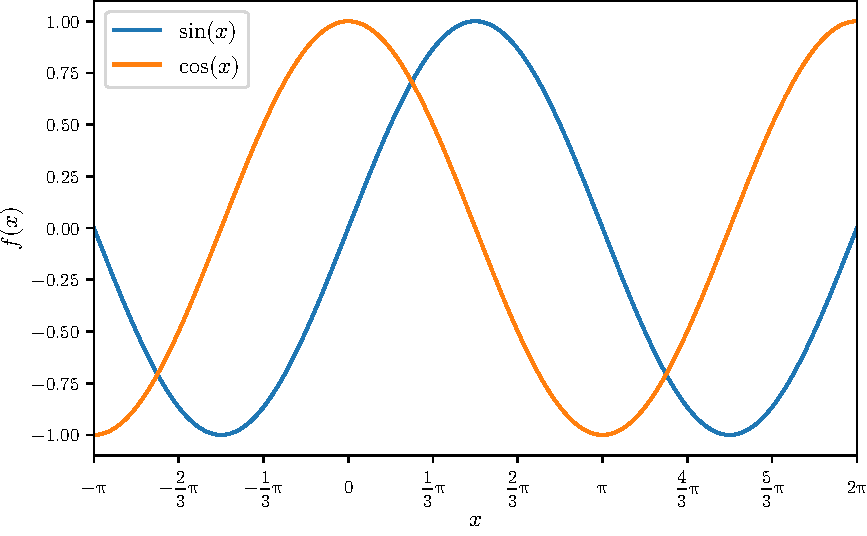
\includegraphics[width=\textwidth]{plot1.pdf}
        \caption{Plot Nummer 1.}
        \label{fig:plot1}
    \end{figure}
    \begin{figure}
        \centering
        \begin{subfigure}{0.48\textwidth}
            \centering
            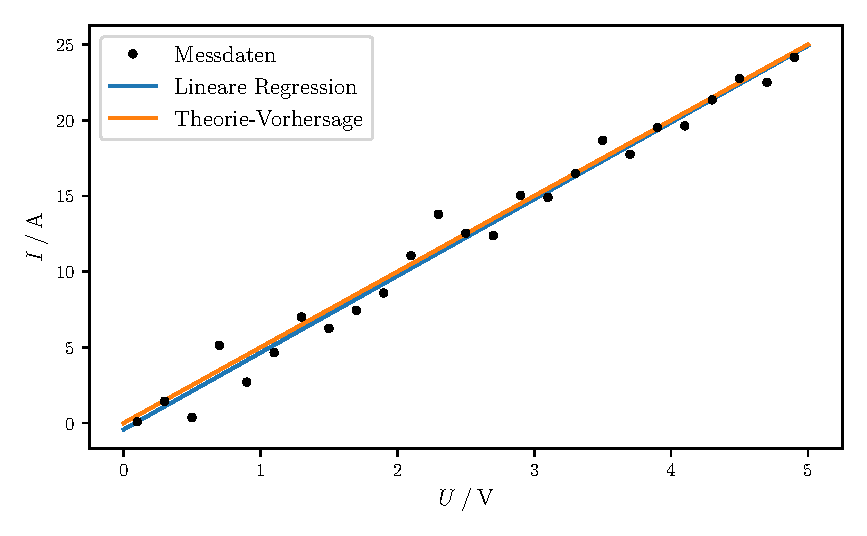
\includegraphics[height=4cm]{plot2.pdf}
            \caption{Lineare Regression.}
            \label{fig:linreg}
        \end{subfigure}
        \begin{subfigure}{0.48\textwidth}
            \centering
            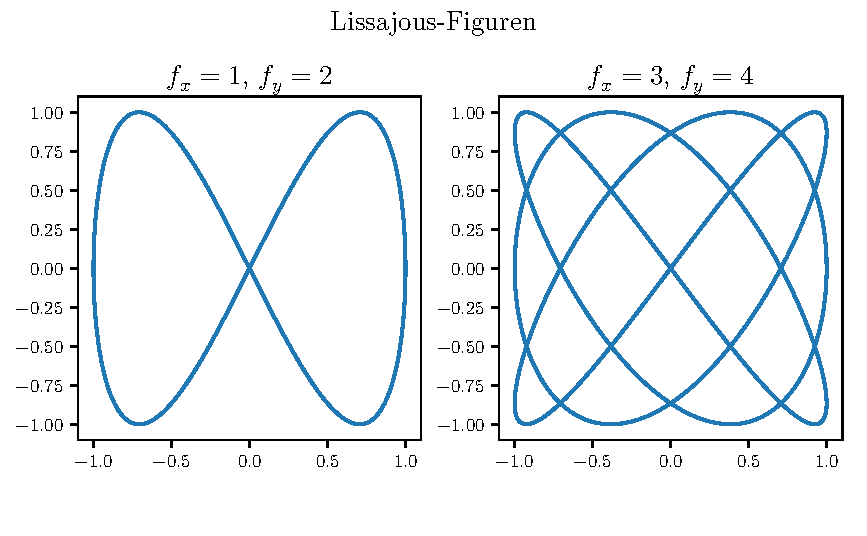
\includegraphics[height=4cm]{plot3.pdf}
            \caption{Lissajous-Figuren.}
            \label{fig:Liss}
        \end{subfigure}
        \caption{Zwei Plots, Abbildung \subref{fig:Liss}: Lissajous-Figuren.}
        \label{fig:logos}
    \end{figure}
\end{document}
